\documentclass[runningheads,a4paper]{llncs}

\usepackage{amssymb}
\setcounter{tocdepth}{3}
\usepackage{graphicx}

\usepackage{url}
\newcommand{\keywords}[1]{\par\addvspace\baselineskip
\noindent\keywordname\enspace\ignorespaces#1}

%%%%%% Added by Wei Liu %%%%%%%
\usepackage{amsmath}
\usepackage[vlined,ruled]{algorithm2e}
\usepackage{lwdefs}
\usepackage{rotating}
%%%%%% End of Added by Wei Liu %%%%%%%

\begin{document}

\mainmatter

\title{Group Analysis of Resting-State fMRI by Hierarchical Markov Random Fields}

\titlerunning{Group fMRI by Hierarchical MRF}

\author{Wei Liu \and Suyash P. Awate\and P. Thomas Fletcher}

\authorrunning{Wei Liu et al.}

\institute{Scientific Computing and Imaging Institute, University of
  Utah, USA, \texttt{weiliu@sci.utah.edu}}

\toctitle{Group Analysis of Resting-State fMRI by Hierarchical Markov Random Fields}

\tocauthor{Wei Liu et al.}

\maketitle

\begin{abstract}
Identifying functional networks from resting-state functional MRI is a
challenging task, especially for multiple subjects. Most current studies
estimate the networks in a sequential approach, i.e., they identify each
individual subject's network independently to other subjects, and then estimate
the group network from the subjects networks. This one-way flow of information
prevents one subject's network estimation benefiting from other subjects. We
propose a hierarchical Markov Random Field model, which takes into account both
the within-subject spatial coherence and between-subject consistency of the
network label map. Both population and subject network maps are estimated
simultaneously using a Gibbs sampling approach in a Monte Carlo Expectation
Maximization framework. We compare our approach to two alternative groupwise
fMRI clustering methods, based on K-means and Normalized Cuts, using both
synthetic and real fMRI data. We show that our method is able to estimate more
consistent subject label maps, as well as a stable group label map.
\end{abstract}


\section{Introduction}
Resting-state functional MRI (rs-fMRI) is widely used for detecting the
intrinsic functional networks of the human brain. The availability of large
rs-fMRI databases opens the door for systematic group studies of functional
connectivity. While the inherently high level of noise in fMRI makes functional
network estimation difficult at the individual level, combining many subjects'
data together and jointly estimating the common functional networks is more
robust. However, this approach does not produce estimates of individual
functional connectivity. Such individual estimates are an important step in
understanding functional networks not just on average, but also how these
networks vary across individuals.

The most common approaches for functional network identification are Independent
Component Analysis (ICA) and its variants
\cite{calhoun2001spatial}, which identify the
statistically independent functional networks without \emph{a priori} knowledge
of the regions of interest. The more recently proposed clustering-based methods
\cite{bellec2010multi,van2008normalized} partition the brain into disjoint
spatial clusters, or label maps, representing the functional networks. Group ICA
\cite{calhoun2001spatial} is a generalization of ICA to multiple subjects, in
which all subjects are assumed to share a common spatial component map but have
distinct time courses. The time courses from all subjects are concatenated
temporally, followed by a single ICA. Although the subject component maps are
obtained by a back-reconstruction procedure, there is no explicit statistical
modeling of the variability between the group and subject component maps.  Ng
et. al \cite{nggroup2012} use group replicator dynamics (RD) to detect subject's
sparse component maps, with group information integrated into each subject's RD
process. In clustering-based methods, the subjects clusterings are usually
averaged to obtain a group affinity matrix and are followed by a second level
clustering on the group similarity matrix
\cite{bellec2010multi,van2008normalized}. Because the group level clustering is
conducted after subject level clustering, the clustering of one subject is
unaware of the information from other subjects, as well as the group clustering.

In this paper we propose a Bayesian hierarchical model to identify the
functional networks from rs-fMRI that includes both subject and population
levels. We assume a group network label map that acts as a prior to the label
maps for all subjects in the population. This Bayesian perspective provides a
natural regularization of the estimation problem of a single subject using
information from the entire population. The variability between the subjects and
group are taken into account through the conditional distributions between group
and subjects. The within-subject spatial coherence is modeled by a Markov Random
Field (MRF). Both the group clustering and subject clusterings are estimated
simultaneously with a Monte Carlo Expectation Maximization (MCEM) algorithm. The
model is data-driven in that all parameters, regularized by two given
hyper-parameters, are estimated from the data, and the only parameter that must
be specified is the number of networks.

Markov Random Fields have previously been used in fMRI analysis to model spatial
context information \cite{descombes1998spatio,liu2010spatial}. However, to our
knowledge, ours is the first hierarchical MRF applied to fMRI for modeling both
group and individual networks. The model of Ng et al. \cite{ng2010group}
combines all subjects into a single MRF and bypasses the need for one-to-one
voxel correspondence across subjects, but the edges are added directly between
subjects without a group layer. In our model, a group layer network map is
explicitly defined, and the consistency between subjects is encoded through
adding edges between group and subjects labels. Our method differs from other
clustering methods \cite{bellec2010multi,van2008normalized} in that their
methods identify the subject's functional network patterns independently,
without any knowledge of other subjects or group population. Instead, our method
estimates both levels of network patterns simultaneously.  The proposed approach
can be seen as a counterpart on the clustering branch of the multi-subject
dictionary learning algorithm \cite{varoquaux2011multi}, which also has a
hierarchical model and a spatially smoothed sparsity prior on the group
component map.

%% One difference between ours and their method is that our subject network map
%% inherently has a spatial smoothness regularization through MRF besides the
%% connection to a smooth group level, while in \cite{varoquaux2011multi} the
%% subject component map's smoothness is encoded only through a sparse and smooth
%% group map.

%We elaborate on the model in section \ref{sec:model}, give the inference
%algorithm in section \ref{sec:inference}, and experiments and discussions in
%section \ref{sec:results}.

\section{Hierarchical Model for Functional Networks}
\label{sec:model}
We define each subject's network label map as a Markov Random Field (MRF) with
statistical dependency between spatially adjacent voxels. These connections act
as a prior model favoring spatial coherence of functional regions. An additional
group label map is defined on top of all subject label maps. The group label map
has the same Markov structure as the individuals, again to encourage spatial
coherence of the functional regions in the group level. In addition, each voxel
in the group is connected to the corresponding voxel of each subject. These
connections model the relationship between the group and the individuals. Hence,
all voxels of subjects and group label map are jointly connected into a single
MRF. See Figure \ref{fig:fig1} for an illustration. More specifically, define a
graph $\cA = (\cS, \cE)$, and the set of node $\cS = (\cG, \cH)$. $\cG$ is the
set of voxels in the group label map, and $\cH = (\cH_1, \dots, \cH_J)$ includes
voxels for all of the $J$ subjects' label maps. An edge $(s, t) \in \cE$ is
defined if 1) $s\in \cH^j, t\in \cG$ and $s$, $t$ are at the same voxel
location, or 2) if $s, t\in \cG$, and $s, t$ are spatial neighbors, or 3) $s,
t\in \cH^j$, and $s, t$ are spatial neighbors. On each node $s \in \cS$, a
random variable $y_s \in \cL = \{1,\cdots, L\}$ is defined to represent the
functional network labels.

\noindent\textbf{MRF Prior: } 
%MRF is a principal method for modeling the spatial context information. Here we
%use it as a prior distribution of network label set $Y$.
Our MRF prior on the hierarchical model is essentially a Potts model with
different weights for the within-subject connections and the connections between
the group and individuals. Because of the equivalence of MRFs and Gibbs fields,
we define our prior as $p(Y) = \frac{1}{Z}\exp\{ -U(Y)\}$, where the energy
function $U(Y)$ is given by
\begin{equation*}
  U(Y) = \sum_{s,r\in\cG} \beta \psi(y_s, y_r) + \sum_{j=1}^J \left ( \sum_{s\in\cG, \tilde s\in\cH^j} \alpha \psi(y_s, y_{\tilde s}) + \sum_{s,r\in\cH^j}\beta\psi(y_s, y_r) \right ).
\end{equation*}
Here $\psi$ is a binary function that is zero when the two inputs are equal and
one otherwise, and $\alpha$ and $\beta$ are parameters determining the strength
of the connections. This regularization encodes two physiologically meaningful
\emph{a priori} assumptions on the functional networks under investigation: 1)
The networks are spatially coherent within single subject. This is modeled by
the $\beta$ term. 2) The networks are similar between subjects, and therefore
between the group and subjects. This is modeled by the $\alpha$ term.  
%The proposed energy function represents both priors without introducing blurring
%artifacts.

\noindent\textbf{Likelihood Model}: In the generative model, for any individual
subject, the observed time course at each voxel is assumed to be generated from
a distribution conditioned on the network label at that voxel. In fMRI analysis
the time series at each voxel is usually normalized to be zero mean and unit
norm, so the analysis is robust to shifts or scalings of the data. This results in the data being projected onto a high-dimensional
unit sphere. After normalization, the sample correlation between two time series
is equal to their inner product.

%% The function connectivity between the time courses of two voxels are independent
%% of their scales and shifts. We normalize the time courses at each voxel to zero
%% mean and unit length. This is equivalent of projecting the data onto a
%% high-dimensional unit sphere. After normalization, the Pearson product
%% correlation between two time courses is equal to their inner product. Therefore
%% the problem of clustering voxels with high correlations can be reformulated to
%% finding clusters with small within-cluster distance on the sphere, where the
%% distance is defined by the inner product of two vectors.

We use the notation $ X = \{ (x_1, \dots, x_N)\, |\, \ x_s \in S^{p-1} \}$
to denote the set of \emph{normalized} time series in $p$-sphere. Given $Y$, the
random vectors $ x_s$ are conditional independent, hence $\log p(
X | Y) = \sum_{s \in \cH} \log p (x_s | y_s)$.  The likelihood function
$p( x_s | y_s)$ is naturally modeled by a von Mises-Fisher (vMF) distribution
\begin{equation}
 f ( x_s| y_s = l; \mu_l, \kappa_l) = C_p(\kappa_l) \exp \left(\kappa_l  \mu_l^T x_s\right),  \quad   x_s \in S^{p-1},  \quad  l \in {\cL},  \label{eq:vmf}
\end{equation}
where for the cluster labeled $l$, $\mu_l$ is the mean direction, $\kappa_l \geq
0$ is the \emph{concentration parameter}, and $C_p$ is the normalization
constant. The larger the $\kappa_l$, the greater the density concentrated around
the mean direction. 

%Since \eqref{eq:vmf} depends on $x$ only by $\mu^T x$, the vMF distribution is
%unimodal and rotationally symmetric around $\mu$.
% May remove the C_p normalization parameter definition since this is really not
% important thing.



\section{Bayesian Inference}
\label{sec:inference}
We solve the inference problem in a \emph{maximum a posteriori} (MAP)
framework. That is, given the observed time course data $X$, we estimate the
posterior mode of $p(Y|X)$. This consists of the following components.

\noindent\textbf{Parameter Estimation: } In this data-driven model, we propose
to estimate the parameters $\theta = \{\alpha, \beta, \kappa, \mu\}$ from the
data using an Expectation Maximization (EM) algorithm. However, the
high-dimensionality and dependency between spatially adjacent voxels in MRF make
it infeasible to obtain a closed form solution of the expectation of $[\log
p(X,Y)]$ with respect to $p(Y|X)$. Here we propose to approximate the
expectation using Monte Carlo EM (MCEM), in which a sample, $(Y^1, \cdots,
Y^M)$, generated from density $p(Y|X)$ is used to approximate the expected value
by the empirical average $\frac{1}{M}\sum_{m=1}^M\log p (X, Y^m)$.

\noindent\textbf{Gibbs Sampling:} Gibbs sampling converts a multivariate
sampling problem into a consecutive univariate sampling, hence is well adapted
to draw the Monte Carlo samples from $p(Y|X)$.  In our hierarchical structure,
the sampling procedure is also done in a hierarchical way. At the image level, a
sample of the group label map, $Y^m_{\cG}$, is drawn given the previous subject
label map, $Y^{m-1}_{\cH_j}$. Next, a sample for each subject map,
$Y^m_{\cH_j}$, is generated given the previous group label map, $Y^{m-1}_{\cG}$.
At the voxel level, we can draw samples of the label $y_s$ given the rest of
nodes fixed, and update $y_s, \forall s \in S$. The conditional probability used
to generate samples at the group and subject voxels are given as
\vspace*{-8pt}
\begin{align}
p(y_s | y_{-s},X) &\propto \frac{1}{Z_s}\exp\{-U(y_s | y_{-s})\} \cdot p(x_s | y_s) = \frac{1}{Z_s}\exp\{-U_p(y_s | y_{\cN_s }, x_s)\} \nonumber\\
U_p &= \alpha\!\sum_{j=1}^J \psi(y_s, y_{\tilde s}^j) + \beta\!\!\sum_{r\in \cN{s}} \psi(y_s,y_r), \quad \forall s \in \cG, \label{eq:sampleg}\\
U_p &= \alpha \psi(y_s,y_{\tilde s}) + \beta\!\!\sum_{r\in \cN{s}} \psi (y_s, y_r) - \kappa_l \mu_l\T x_s - \log C_p, \: \forall s \in \cH_j, \label{eq:sampleh}
\end{align}
where $-s$ is the set of all nodes excluding $s$, $Z_s$ the normalization constant, $U_p$ is the posterior energy,
and $\cN_s$ is the set of neighbor's of $s$. In our model we use 6-neighbor
system in a 3D volume image.  $y_{\tilde s}^j$ in \eqref{eq:sampleg} is the
label of subject $j$'s voxel with the same spatial location with $s$, and
$y_{\tilde s}$ in \eqref{eq:sampleh} is the label of group's voxel with the same
spatial location with $s$. Because of the dependency on previous samples, the
sequence of samples will be a Markov Chain, hence our method falls into Markov
Chian Monte Carlo (MCMC) sampling.  After a sufficient burn-in period, a series
of samples $Y^m, m = 1\cdots M$ is saved for approximating the expectation
$\mathbb{E}[\log p(X,Y)]$.

\noindent \textbf{Pseudo likelihood: } To evaluate $\log p(X,Y^m;\theta) = \log
p(Y^m;\theta) + \log p(X|Y^m;\theta)$ as a function of $\theta$, we face the
difficulty of evaluating the partition function $Z$ in $p(Y^m)$.  In practice the
Gibbs field is approximated by pseudo-likelihood, which is defined as the
product of the conditional distribution $p(y_s|y_{-s}), \forall s \in
\cS$. Therefore the energy function can be written as
\begin{align*}
U(Y) &\approx  \sum_{s\in\cS} U(y_s | y_{-s}) = \sum_{s\in\cG} \left ( \alpha \sum_{j\in J} \psi(y_s,y_{\tilde s}^j) +\beta\sum_{r\in \cN{s}} \psi(y_s, y_r) \right ) \\
&+ \sum_{j=1}^J \sum_{s\in\cH^j} \left (\alpha \psi(y_s, y_{\tilde s}) + \beta \sum_{r\in \cN_s} \psi(y_s, y_r) \right ),
\end{align*}
where $y_{\tilde s}^j$ and $y_{\tilde s}$ has the same definition with \eqref{eq:sampleg} and \eqref{eq:sampleh}.

\noindent\textbf{Hierarchical MRF algorithm using MCEM: } With all the
preparation above, parameter estimation can be done by maximizing
$\frac{1}{M}\sum_{m=1}^M\log p (X, Y^m)$. The $\alpha$ and $\beta$ in the MRF
prior can be optimized by maximizing $\frac{1}{M}\sum_{m=1}^M\log p (Y^m)$ with
a Newton-Raphson method. We assume a Gaussian prior distribution on $\alpha$
with hyper-parameters $\mu_{\alpha}$ and $\sigma_{\alpha}$, which is given manually and does not have significant impact on the model. In order for MCMC
sampling to converge quickly to the posterior, we need a reasonably good initial network label map. Here the K-means clustering on a concatenated group dataset
is used for the initial maps of both the group and subjects. After the EM
parameter estimation iterations are done, an Iterated Conditional Modes (ICM) on
the current sample map gives the final label maps. Putting this all together,
the \textsf{groupmrf} algorithm to estimate the group and individual label maps
is given in Algorithm \ref{alg:alg1}.
\vspace*{-16pt}
\begin{algorithm}[htb]
  \label{alg:alg1}
  %% \SetAlgoLined
  \KwData{Normalized fMRI, initial group label map}
  \KwResult{Group label map $Y_{\cG}$, subjects label map $Y_{\cH}$, parameters $\{\alpha, \beta, \mu, \sigma\}$}
  \While{$\mathbb{E}[\log p(X, Y)]$ not converge}{
    %% E step\;
    \Repeat{$B+M$ times}{
      \lForEach(){$s \in \cG$}{
        Draw consecutive samples of $y_s$ from $p(y_s | y_{\cN_s}, X;\theta)$ using \eqref{eq:sampleg}
      }
      \ForEach(){$j  = 1\dots J$}{
        \lForEach(){$s \in \cH_j$}{
        Draw consecutive samples of $y_s$ from $p(y_s | y_{\cN_s}, X; \theta)$ using \eqref{eq:sampleh}
        }
      }
      Save sample $Y^m $ after $B$ burn-ins\;
    }
    %% M step\;
    \ForEach{$l = 1\cdots L$} {
      Estimate $\{\mu_l, \kappa_l\}$ by maximizing $\frac{1}{M}\sum_{m=1}^M\log p (X|Y^m)$\;
    }
    Estimate $\{\alpha, \beta\}$ by maximizing $\frac{1}{M}\sum_{m=1}^M\log p (Y^m)$\;
  }
  Run ICM on current samples to estimate final label maps.
  \caption{Monte Carlo EM for group MRF}
\end{algorithm}
\vspace*{-20pt}
\section{Results and Conclusion}
\label{sec:results}

Three methods are compared in both  synthetic data and \emph{in vivo} data
test. The first method is \textsf{K-Means} \cite{bellec2010multi} applied on
each subject's fMRI data, as well as on a group dataset constructed by
concatenating all subjects time courses. To alleviate the dependency on initial
cluster centers, we run \textsf{K-Means} 20 times with different initial cluster
centers generated by a \textsf{K-means++} algorithm. The second method is a
Normalized-Cuts algorithm (\textsf{N-Cuts}), following Van den Heuvel, et
al.~\cite{van2008normalized}, which is applied in two stages. First N-Cuts is
run on each subject's affinity matrix, as computed by pairwise
correlation between time courses. Second, N-Cuts is applied on a group affinity
matrix, which is computed by summing up all of the subjects' segmentation
matrices. We use the \textsf{Ncutclustering\_9} toolbox
\cite{shi2000normalized}, a newer version of the one used in
\cite{van2008normalized}. The third method is our \textsf{groupmrf} approach
applied on all subjects' fMRI data. The preprocessing are same for all three
methods except that \textsf{groupmrf} use image data without spatial smoothing,
while the other two use data smoothed by a standard 6mm Gaussian filter.
\vspace*{-8pt}
\begin{figure}[htb]
  \begin{tabular}[b]{c}
    \includegraphics[width=0.35\textwidth]{figure1/grp2}
  \end{tabular}
  \hspace{5pt}
  \begin{tabular}[b]{c}
    \begin{tabular}[b]{lccccc}
      & \footnotesize Truth & \footnotesize \textsf{K-Means} & \footnotesize \textsf{N-Cuts} & \footnotesize \textsf{groupmrf}\\
      \begin{sideways} \footnotesize group \end{sideways} &
      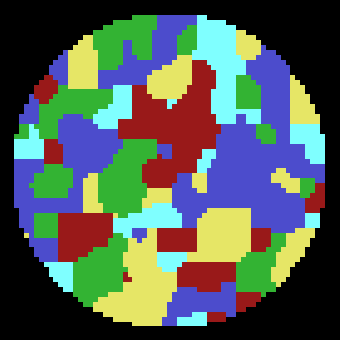
\includegraphics[width=0.12\textwidth]{figure1/truegrp} &
      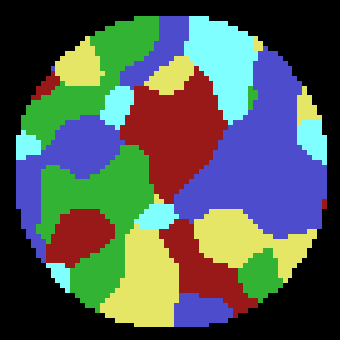
\includegraphics[width=0.12\textwidth]{figure1/kmeans_grp} &
      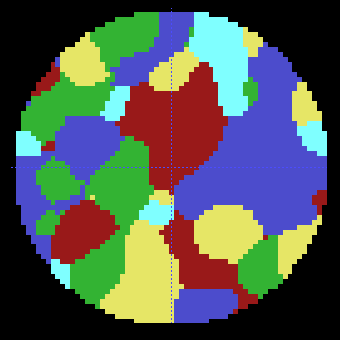
\includegraphics[width=0.12\textwidth]{figure1/ncuts_grp} &
      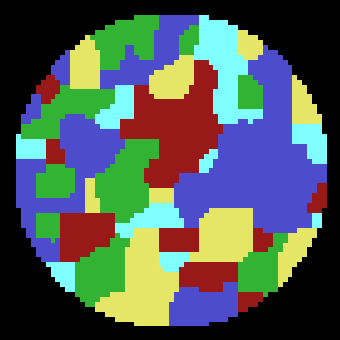
\includegraphics[width=0.12\textwidth]{figure1/mrf_grp} \\
      \begin{sideways} \footnotesize sub 1 \end{sideways} &
      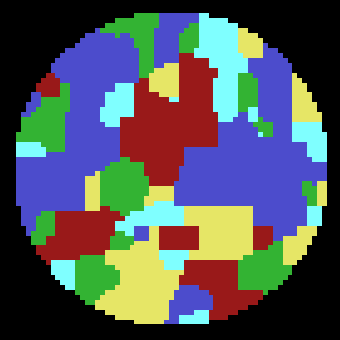
\includegraphics[width=0.12\textwidth]{figure1/true_sub1} &
      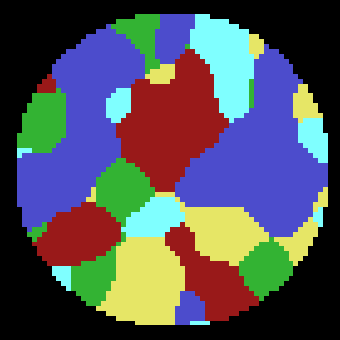
\includegraphics[width=0.12\textwidth]{figure1/kmeans_sub1} &
      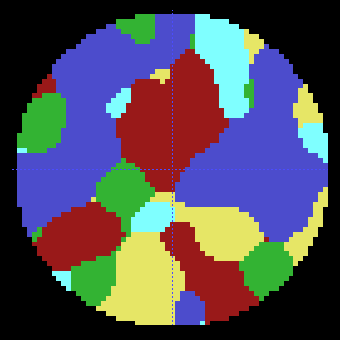
\includegraphics[width=0.12\textwidth]{figure1/ncuts_sub1} &
      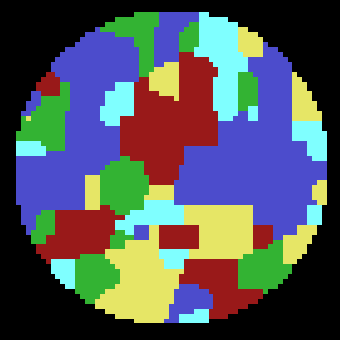
\includegraphics[width=0.12\textwidth]{figure1/mrf_sub1} \\
    \end{tabular} \\
    \hspace{15pt}
    \footnotesize
    \begin{tabular}[b]{l|ccc}
      & group & mean(sub) & var(sub) \\
      \textsf{K-means} & 92.9 & 87.0 & 0.67\\
      \textsf{N-Cuts} & 85.4 & 87.1 & 0.58 \\
      \textsf{groupmrf} & 95.7 & 97.5 & 0.59
    \end{tabular}
  \end{tabular}
  \caption{Left: Hierarchical MRF depicted by undirected graph. The $J$ subjects
    are compactly represented by a box with label $J$. Right: clustering of
    \textsf{K-means} and \textsf{N-Cuts} on synthetic time series with spatial
    smoothing, and \textsf{groupmrf} without smoothing. Top is group label map
    and bottom is one of subjects label map. The table gives the rand index accuracy
    between estimated label map and ground truth image. The rand index of all
    subjects are summarized by a mean and variance value.}
  \label{fig:fig1}
\vspace*{-8pt}
\end{figure}

\noindent\textbf{Synthetic example:} We simulate synthetic time course on each
voxel of 16 subjects by first sampling from MRF with $\alpha = 0.4$ and $\beta =
2.0$ and get both group and subjects network label map. The time course signals
at each voxel are generated by adding Gaussian white noise of $\sigma^2 = 40$ on
each cluster's mean time course, which is synthesized from an auto-regressive
process of $x_t = \varphi x_{t-1} + \varepsilon$ with $\varphi = 0.7$ and noise
variance $\sigma_{\varepsilon} = 1$. The sample correlation between the mean
time series is in the range of $(-0.15, 0.3)$. The rand index value on right
side of Figure \ref{fig:fig1} shows that \textsf{groupmrf} algorithm is able to
detect both group and subjects label map more accurately than the
\textsf{K-Means} and \textsf{N-Cuts} method. The synthetic images shows that
despite the different assumption of \textsf{K-Means} and \textsf{N-cuts} on the
data, our algorithm is able to estimate subject label maps with more spatial and
inter-subject coherence than the other two methods.

\begin{figure}[htb]
\centering
\begin{tabular}{lcc|cc|cc}
&
\multicolumn{2}{c|}{group} &
\multicolumn{2}{c|}{sub 1} &
\multicolumn{2}{c}{sub 2} \\
& $z = 26$ & $z=54$ & $z = 26$ & $z=54$ & $z = 26$ & $z=54$ \\
\begin{sideways} \footnotesize \textsf{K-Means} \end{sideways} &
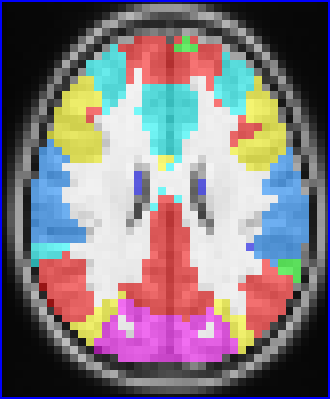
\includegraphics[width=0.15\textwidth]{figure2/kmeans_grp_z25} &
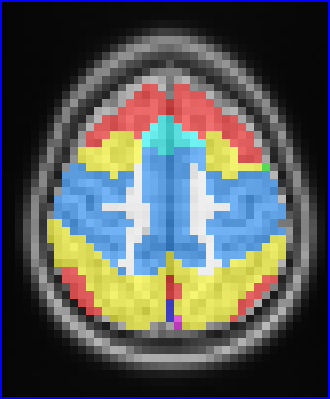
\includegraphics[width=0.15\textwidth]{figure2/kmeans_grp_z32} &
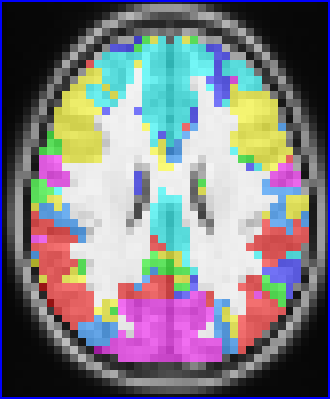
\includegraphics[width=0.15\textwidth]{figure2/kmeans_sub1_z25} &
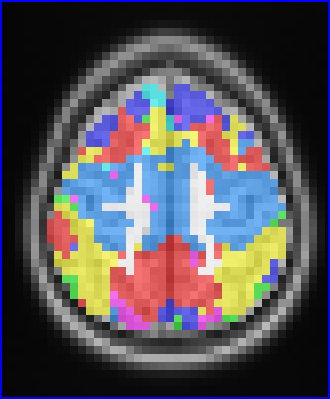
\includegraphics[width=0.15\textwidth]{figure2/kmeans_sub1_z32} &
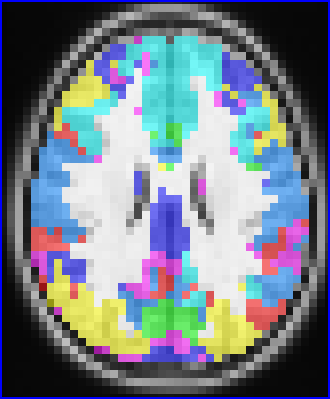
\includegraphics[width=0.15\textwidth]{figure2/kmeans_sub2_z25} &
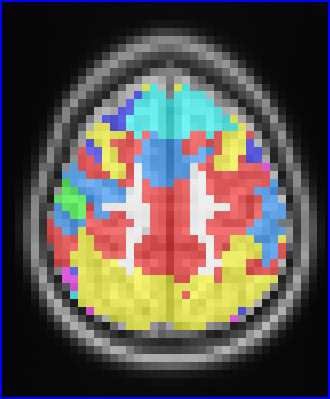
\includegraphics[width=0.15\textwidth]{figure2/kmeans_sub2_z32} \\
\begin{sideways} \footnotesize \textsf{N-Cuts} \end{sideways} &
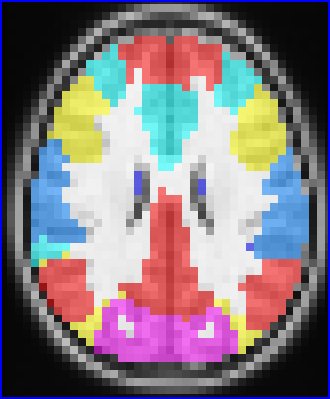
\includegraphics[width=0.15\textwidth]{figure2/ncuts_grp_z25} &
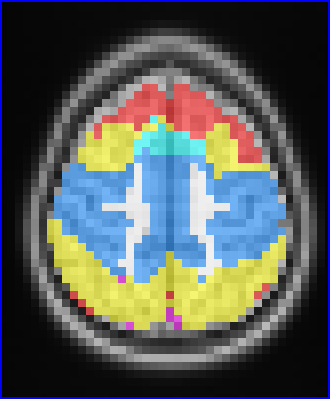
\includegraphics[width=0.15\textwidth]{figure2/ncuts_grp_z32} &
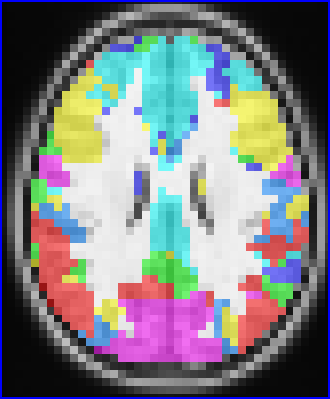
\includegraphics[width=0.15\textwidth]{figure2/ncuts_sub1_z25} &
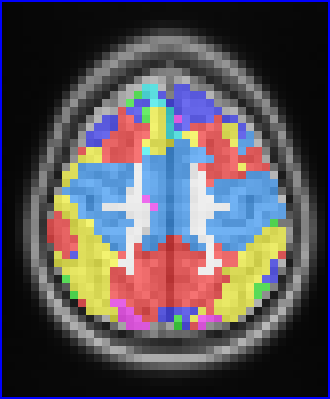
\includegraphics[width=0.15\textwidth]{figure2/ncuts_sub1_z32} &
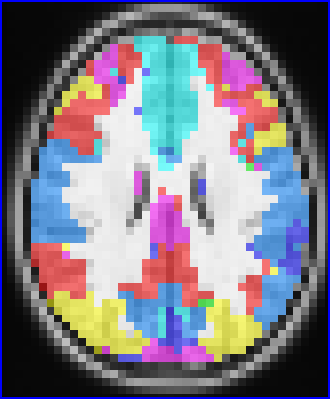
\includegraphics[width=0.15\textwidth]{figure2/ncuts_sub2_z25} &
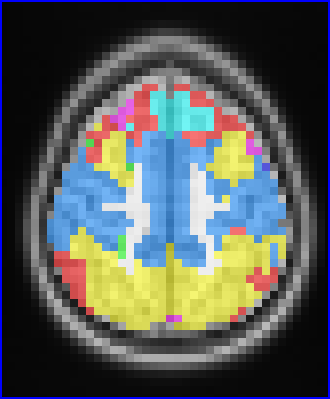
\includegraphics[width=0.15\textwidth]{figure2/ncuts_sub2_z32} \\
\begin{sideways} \footnotesize \textsf{groupmrf} \end{sideways} &
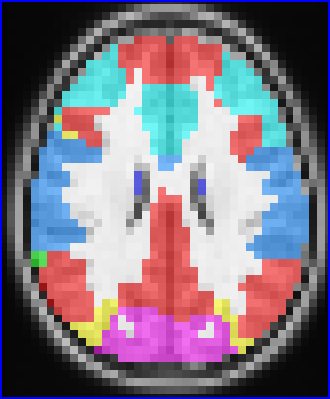
\includegraphics[width=0.15\textwidth]{figure2/mrf_grp_z25} &
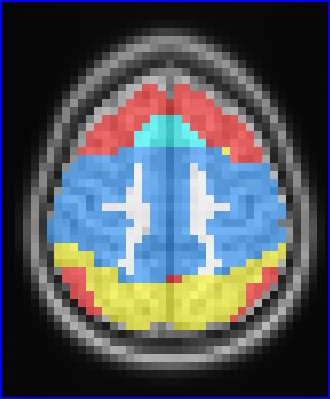
\includegraphics[width=0.15\textwidth]{figure2/mrf_grp_z32} &
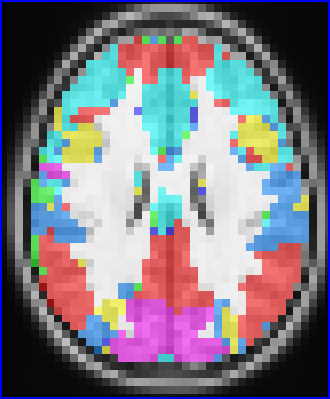
\includegraphics[width=0.15\textwidth]{figure2/mrf_sub1_z25} &
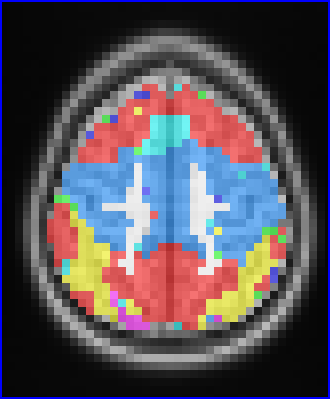
\includegraphics[width=0.15\textwidth]{figure2/mrf_sub1_z32} &
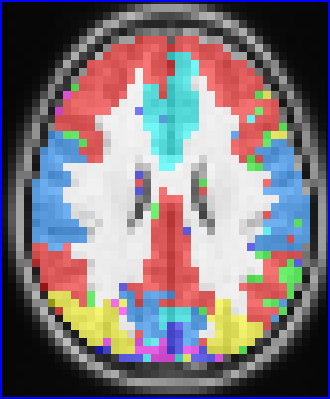
\includegraphics[width=0.15\textwidth]{figure2/mrf_sub2_z25} &
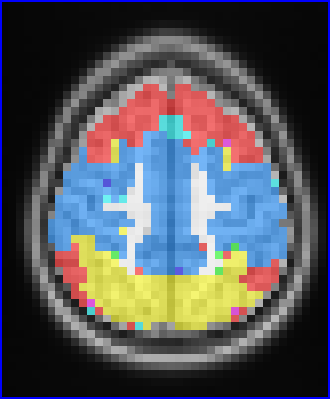
\includegraphics[width=0.15\textwidth]{figure2/mrf_sub2_z32}
\end{tabular}
\caption{Functional networks estimated by 3 methods shown in separate rows. \textsf{groupmrf} has more consistent estimation of the DMN (red) and motor network (blue) among two example subjects of 66 total used.}
\vspace*{-8pt}
\label{fig:fig2}
\end{figure}

\noindent\textbf{In vivo Data} We tested our method on the ADHD-200 dataset in the
1000 Functional Connectomes Project. A total of 66 healthy control adolescent
subjects were chosen from the same site (University of Pittsburgh). BOLD EPI
images (TR = 1.5 s, TE = 29 ms, 29 slices at 4 mm slice thickness, 64 x 64
matrix, 196 volumes) were acquired on a Siemens 3 Tesla Trio scanner. The fMRI
volumes were motion corrected, slice timing corrected, registered to NIHPD
object 1 atlas, bandpass filtered to 0.01 to 0.1 Hz, regressed out nuisance
variables including white matter, CSF mean time courses and six motion
parameters, and at last filtered by a 8 mm Gaussian filter for spatial
smoothness.

Figure \ref{fig:fig2} shows the functional networks computed from the three
methods. As in the synthetic data experiment, all 66 subjects' time series were
concatenated into a single group dataset. \textsf{K-means} and \textsf{N-Cuts}
were applied on the spatially-smoothed, concatenated group dataset, as well as
on each subject fMRI. Our \textsf{groupmrf} was applied on all subjects data
without any spatial smoothing and with the initial parameter values $\alpha =
0.7, \beta = 1.0$. Following \cite{van2008normalized,bellec2010multi}, the
number of clusters are set to 7. It can be seen in Figure \ref{fig:fig2} that
our algorithm is able to detect the major functional networks even for
individual subjects, while \textsf{K-means} and \textsf{N-Cuts} miss some
components in the Default Mode Network (DMN) for certain subjects, due to the
high noise level of single subject data.

\begin{figure}[htb]
\centering
\begin{tabular}[b]{cc|cc|cc}
\multicolumn{2}{c}{sub1} &
\multicolumn{2}{c}{sub2} &
\multicolumn{2}{c}{sub3} \\
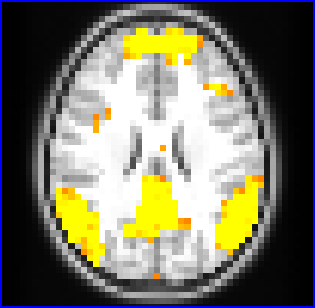
\includegraphics[width=0.15\textwidth]{figure3/dmn_a} &
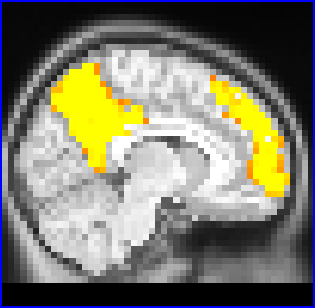
\includegraphics[width=0.15\textwidth]{figure3/dmn_s} &
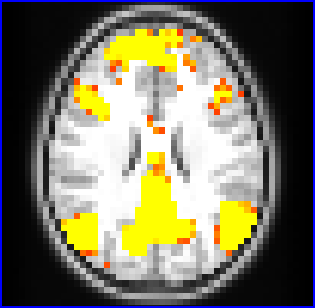
\includegraphics[width=0.15\textwidth]{figure3/dmn_sub17_a} &
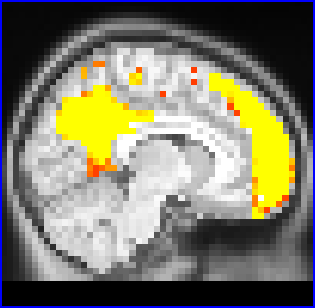
\includegraphics[width=0.15\textwidth]{figure3/dmn_sub17_s} &
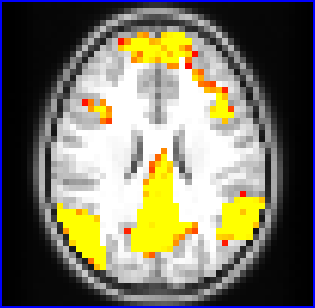
\includegraphics[width=0.15\textwidth]{figure3/dmn_sub21_a} &
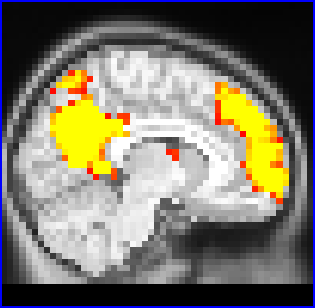
\includegraphics[width=0.15\textwidth]{figure3/dmn_sub21_s} \\
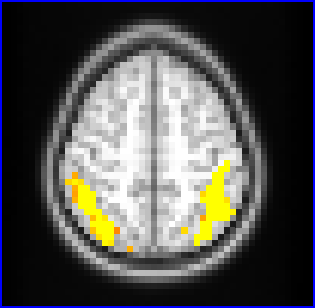
\includegraphics[width=0.15\textwidth]{figure3/atten_a} &
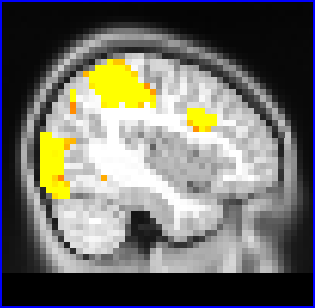
\includegraphics[width=0.15\textwidth]{figure3/atten_s} &
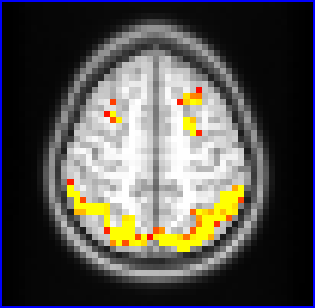
\includegraphics[width=0.15\textwidth]{figure3/atten_sub17_a} &
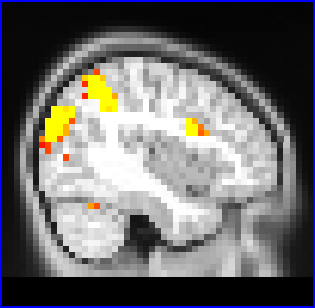
\includegraphics[width=0.15\textwidth]{figure3/atten_sub17_s} &
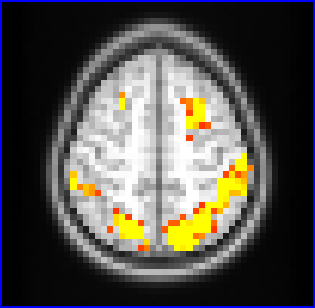
\includegraphics[width=0.15\textwidth]{figure3/atten_sub21_a} &
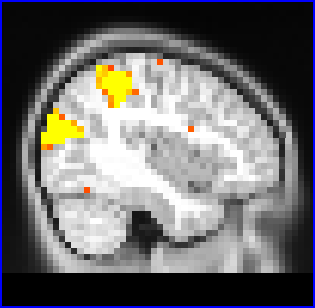
\includegraphics[width=0.15\textwidth]{figure3/atten_sub21_s} 
\end{tabular}

\includegraphics[width=0.03\textwidth]{figure3/colorbar}
\caption{Posterior probability maps of DMN and attention network for 3 example
  subjects out of the 66 total used. Top row: DMN, $x = -8, z=26$. Bottom row:
  attention network. $x=40, z=54$.}
\label{fig:fig3}
\end{figure}

The real strength of Bayesian statistics lies in the probabilistic explanation of
the results. The last experiment in Figure \ref{fig:fig3} shows the posterior
probability maps of DMN and attention network of two subjects. The maps are approximated by averaging the Monte-Carlo samples from the individual
posterior densities. Unlike other approaches, such as ICA or clustering,
these images provide a truly probabilistic interpretation of a voxel's
membership in a particular network.

%% This is \cite{craddock2012}

\noindent{\bf Acknowledgment: } This work is supported by NIH Roadmap for Medical Research, Grant U54-EB005149 (NAMIC), and NIH CIBC grant P41-RR12553. 
\bibliographystyle{splncs03}
\bibliography{ref}
\end{document}
